\chapter{\babTiga}
\label{bab:3}

This chapter presents the system design and methodology for the development of custom descheduler plugin policies. It provides a high-level overview of the system architecture and illustrates the operational flow of the proposed policies. Section 3.1 and its subsections describe the design of the Imbalance Index balancing policy, including its mathematical formulation for computing cluster imbalance, execution workflow, and the expected YAML configuration. Section 3.2 and its subsections discuss the design and architecture of the Network-Aware Evictor policy, focusing on the tools used to obtain latency data, its operational workflow, and the corresponding YAML configuration.

\section{TOPSIS-RDG: Resource Defragmentation}
\label{sec:topsis_rdg}
The implementation of the new introduced Resource Defragmentation kubernetes descheduler plugin adapts the Resource Defragmentation Greedy (RDG) strategy from the provided research  but enhances it using a TOPSIS (Technique for Order of Preference by Similarity to Ideal Solution) multi-criteria decision-making framework to evaluate eviction candidates.

\subsection{Execution Flow of Resource Defragmentation}
\label{sec:execution_flow}
The execution flow of the \texttt{ResourceDefragmentation} plugin is divided into two primary phases: Fragmentation Detection and the Eviction Loop. This process ensures that the descheduler evaluates the cluster dynamically and minimizes unnecessary evictions.

\begin{itemize}
    \item \textbf{Phase 1: Fragmentation Detection} \\
    During the initial setup of the \texttt{Balance} extension point, the plugin detects and profiles the imbalance across the cluster.
    \begin{itemize}
        \item \textbf{Cache Initialization:} The descheduler iterates over all nodes in the cluster and retrieves the pods currently running on them. It utilizes a pre-configured \texttt{podFilter} to ignore non-evictable workloads (e.g., DaemonSets, static pods, or excluded namespaces).
        \item \textbf{Node Profiling:} It calculates the total allocatable and currently requested CPU and memory for each node.
        \item \textbf{Threshold Check:} The plugin computes the Resource Imbalance Index (RII) for each node. If the absolute value of the node's RII exceeds the configured \texttt{ImbalanceThreshold}, the node is flagged as ``fragmented''.
        \item \textbf{Prioritization:} For every fragmented node, the system calculates the Free Space Index (FSI) and combines it with the RII to generate a \texttt{priorityIndex}. The nodes are then sorted in descending order, ensuring that the most severe offenders are processed first.
    \end{itemize}

    \item \textbf{Phase 2: The Eviction Loop} \\
    The plugin enters an eviction loop constrained by the \texttt{MaxEvictions} parameter, systematically addressing the prioritized fragmented nodes.
    \begin{itemize}
        \item \textbf{Candidate Selection (TOPSIS):} Starting with the most severely fragmented node, all running pods on the node are passed into the TOPSIS evaluation function. The pods are evaluated against the four criteria ($C_1$, $C_2$, $C_3$, and $C_4$). The pod that achieves the highest Closeness Coefficient (CC) is selected as the mathematically optimal candidate for eviction.
        \item \textbf{Execution:} The plugin hands the selected candidate pod to the framework's evictor API.
        \item \textbf{Dynamic State Re-evaluation:} To prevent over-eviction and avoid waiting for the Kubernetes APIServer to reconcile, the plugin immediately evaluates the outcome if the eviction succeeds:
        \begin{itemize}
            \item The local memory cache (\texttt{nodeStates}) is updated by subtracting the evicted pod's CPU and memory requests from the node's total requested resources.
            \item The node's RII is recalculated based on the updated cache.
            \item \textbf{Queue Management:} If the new RII falls below the threshold, the node is considered ``healed'' and is removed from the \texttt{fragmentedNodes} queue. If the node remains imbalanced, the evicted pod is removed from the local slice, and the node is kept in the queue for potential further evictions in subsequent iterations.
        \end{itemize}
    \end{itemize}
\end{itemize}

\subsection{TOPSIS-Based Resource Defragmentation Algorithm}
\label{sec:topsis_algorithm}

The core of the \texttt{ResourceDefragmentation} plugin is an enhancement of the Resource Defragmentation Greedy (RDG) strategy proposed by Guo et al. \cite{guo2025joint}. While the original RDG algorithm relies on a greedy correlation metric to select migration candidates, this implementation introduces a Technique for Order of Preference by Similarity to Ideal Solution (TOPSIS) framework to evaluate multiple dimensions of an eviction's impact.

To understand the criteria, we must first establish the foundational metric defined in the RDG approach: the Resource Imbalance Index (RII) \cite{guo2025joint}. The RII quantifies the disparity between CPU and memory utilization, identifying whether a node or container is disproportionately consuming one resource over the other. 
For a node $i$, the RII is calculated as:
\begin{equation}
    RII_i = \frac{\sum_{j=1}^{n} r_c(j)}{R_c} - \frac{\sum_{j=1}^{n} r_m(j)}{R_m}
\end{equation}
where $r_c(j)$ and $r_m(j)$ are the requested CPU and memory of pod $j$, and $R_c$ and $R_m$ are the total allocatable capacities of the node. The RII evaluates to a domain of $(-1, 1)$, where a higher absolute value indicates severe dimensional fragmentation (e.g., a highly positive value means CPU is exhausted while memory remains stranded). The RII of a single container/pod $j$ is calculated similarly using its individual requests against the node's capacity.

The decision-making algorithm operates through the following formalized stages:

\begin{enumerate}
    \item \textbf{Fragmentation Detection and Prioritization:} \\
    For each node $i$ in the cluster, the algorithm calculates $RII_i$ and the Free Space Index ($FSI_i$) to quantify resource disparity and stranded capacity \cite{guo2025joint}. Nodes with an absolute $RII_i$ exceeding the configured threshold are flagged as fragmented. 
    
    To determine the processing order, these nodes are sorted in descending order based on their Priority Index \cite{guo2025joint}:
    \begin{equation}
        \text{Priority}_i = w_p \cdot |RII_i| + \left(1 - w_p\right) \cdot \frac{1}{FSI_i + \epsilon}
        \label{eq:priority_index}
    \end{equation}
    where $\epsilon$ ($1e^{-10}$) is a small constant to prevent division by zero.

    \item \textbf{Multi-Criteria Candidate Evaluation:} \\
    For a prioritized fragmented node, every running pod $j$ is evaluated against four distinct criteria to build an $n \times 4$ decision matrix $X$. The first three criteria mathematically map to the goals of resource defragmentation:
    \begin{itemize}
        \item \textbf{$C_1$: Imbalance Alignment (Benefit).} Derived directly from the migration priority correlation metric in \cite{guo2025joint}, this criterion measures the degree to which a pod's specific resource demands exacerbate the host node's overall imbalance. A higher positive value indicates that evicting this pod will forcefully correct the node's skew.
        \begin{equation}
            C_1 = RII_i \cdot RII_j \cdot \max\left( \frac{r_c(j)}{R_c}, \frac{r_m(j)}{R_m} \right)
        \end{equation}
        
        \item \textbf{$C_2$: Target Node Improvement (Benefit).} This criterion simulates the broader cluster impact if the pod is migrated. It iterates through all other nodes $k$ in the cluster that have enough free space to host pod $j$. It calculates the maximum potential reduction in fragmentation across the cluster by finding the target node where the pod's arrival actually heals existing imbalance:
        \begin{equation}
            C_2 = \max_{k \neq i} \left( |RII_k| - |RII_k'| \right)
        \end{equation}
        where $RII_k'$ is the simulated imbalance of node $k$ after receiving pod $j$. If the pod cannot fit on any other node, $C_2$ is heavily penalized.
        
        \item \textbf{$C_3$: Free Space Expansion (Benefit).} While $C_1$ fixes the dimensional ratio, $C_3$ prioritizes the raw volume of contiguous space recovered. Let $c$ and $m$ be the current available CPU and memory ratios of node $i$, and $p_c$ and $p_m$ be the pod's requested resource ratios. The initial free space area of the node is defined as $F_i = c \cdot m$. If the pod is evicted, the new free space area becomes $F_i' = (c + p_c) \cdot (m + p_m)$. $C_3$ mathematically measures the exact expansion of the node's normalized Free Space Area ($\Delta F_i$) through the following derivation:
        \begin{equation}
            \begin{aligned}
                \Delta F_i &= F_i' - F_i \\
                \Delta F_i &= (c + p_c) \cdot (m + p_m) - (c \cdot m) \\
                \Delta F_i &= (c \cdot m) + (c \cdot p_m) + (m \cdot p_c) + (p_c \cdot p_m) - (c \cdot m) \\
                C_3 &= \Delta F_i = c \cdot p_m + m \cdot p_c + p_c \cdot p_m
            \end{aligned}
        \end{equation}
        
        \item \textbf{$C_4$: Pod Priority Penalty (Cost).} Evaluates the Kubernetes priority class of the pod. In the TOPSIS matrix, this is treated as a cost, ensuring the algorithm naturally avoids evicting critical system workloads.
    \end{itemize}

    \item \textbf{TOPSIS Closeness Coefficient Calculation:} \\
    The decision matrix $X$ undergoes vector normalization and is multiplied by a predefined weight vector $W = [0.30, 0.30, 0.25, 0.15]$. The Euclidean distances from the Ideal Best ($D_j^+$) and Ideal Worst ($D_j^-$) solutions are computed for each pod. Finally, the relative closeness coefficient ($CC_j$) is calculated:
    \begin{equation}
        CC_j = \frac{D_{j}^{-}}{D_{j}^{+} + D_{j}^{-}}
        \label{eq:closeness_coefficient}
    \end{equation}
    The pod with the highest $CC_j$ represents the mathematical optimum for eviction.

    \item \textbf{Dynamic State Re-evaluation:} \\
    Upon a successful eviction, the node's requested resources are immediately decremented in the plugin's local cache, and its $RII_i$ is dynamically recalculated. If the $|RII_i|$ falls below the acceptable threshold, the node is considered ``healed'' and is removed from the processing queue.
\end{enumerate}

\subsection{Justification for Algorithm Weights}
\label{sec:algorithm_weights}

The effectiveness of the TOPSIS-RDG algorithm relies on the careful tuning of the node Priority Index weight ($w_p$) and the TOPSIS criteria weight vector ($W$).

\textbf{Priority Index Weight ($w_p = 0.5$):} 
In Equation \ref{eq:priority_index}, $w_p$ dictates the relative importance of correcting dimensional resource imbalance ($|RII_i|$) versus alleviating absolute resource exhaustion (the inverse of the Free Space Index). We assign $w_p = 0.5$ to establish an equal balance. If $w_p$ approached $0$, the algorithm would blindly chase highly utilized nodes (causing unnecessary churn, similar to the default \textit{HighNodeUtilization} policy). If $w_p$ approached $1$, it might target mostly-empty nodes that happen to have a skewed CPU-to-memory ratio, wasting evictions without freeing up meaningful capacity. A balanced weight explicitly targets the intersection of both problems: nodes that are dangerously full \textit{and} highly skewed.

\textbf{TOPSIS Criteria Weights ($W = [0.30, 0.30, 0.25, 0.15]$):}
The weight vector in the TOPSIS matrix reflects the strategic priorities of the descheduler:
\begin{itemize}
    \item $C_1$ (30\%) and $C_2$ (30\%) receive the highest weighting because the primary objective of this plugin is multidimensional defragmentation. Resolving local host skew ($C_1$) and ensuring the pod heals a target host upon rescheduling ($C_2$) are critical to preventing scheduling deadlocks.
    \item $C_3$ (25\%) acts as a secondary objective. While recovering large contiguous blocks of free space is important, it should not overshadow the need for dimensional alignment.
    \item $C_4$ (15\%) acts as a safety penalty. The lower weight allows priority to act as a tie-breaker, ensuring the descheduler does not bypass an objectively perfect defragmentation candidate just because it has a slightly elevated priority, while still fiercely protecting maximum-priority system-critical pods.
\end{itemize}

% TODO: Justifikasi, kenapa pake Wp 0,5, kenapa pake W = [0.30, ...]

\subsection{Illustrative TOPSIS Evaluation Scenario}
\label{sec:topsis_example}

To clarify the practical application of the TOPSIS criteria, Table \ref{tab:topsis_example} presents a hypothetical scenario. Consider a severely fragmented node (\texttt{Node-A}) that is experiencing CPU exhaustion but possesses abundant unused memory ($RII_A \gg 0$). The algorithm evaluates three candidate pods currently running on this node to determine the optimal eviction target.

The candidate pods are characterized as follows:
\begin{itemize}
    \item \textbf{Pod 1 (CPU-Heavy, Best-Effort):} Its resource profile aligns precisely with the node's bottleneck. Moving it will drastically improve the node's balance and free up the constrained CPU resource. It has a low Kubernetes priority.
    \item \textbf{Pod 2 (Memory-Heavy, Best-Effort):} Evicting this pod would remove memory (which the node already has in excess) rather than CPU, effectively worsening the node's dimensional imbalance.
    \item \textbf{Pod 3 (CPU-Heavy, System-Critical):} While mathematically ideal for rebalancing the node, it belongs to a critical system component with an extremely high priority class.
\end{itemize}

\begin{table}[htbp]
    \centering
    \caption{Hypothetical TOPSIS Decision Matrix for Candidate Pods on \texttt{Node-A}}
    \label{tab:topsis_example}
    \renewcommand{\arraystretch}{1.3} % Adds slightly more vertical padding
    \begin{tabular}{l c c c c | c}
        \hline
        \textbf{Candidate Pod} & \textbf{$C_1$: Imbalance} & \textbf{$C_2$: Target Node} & \textbf{$C_3$: Free Space} & \textbf{$C_4$: Priority} & \textbf{Final Score} \\
        & \textbf{Alignment (+)} & \textbf{Improvement (+)} & \textbf{Expansion (+)} & \textbf{Penalty (-)} & \textbf{($CC_i$)} \\
        \hline
        \textbf{Pod 1} (Ideal)   & $0.45$  & $0.20$ & $0.35$ & $100$     & \textbf{$0.88$} \\
        \textbf{Pod 2} (Mismatch)& $-0.10$ & $0.05$ & $0.15$ & $100$     & $0.22$ \\
        \textbf{Pod 3} (Critical)& $0.50$  & $0.20$ & $0.40$ & $10,000$  & $0.05$ \\
        \hline
    \multicolumn{6}{l}{\small \textit{(+) indicates a Benefit criterion; (-) indicates a Cost criterion.}} \\
    \end{tabular}
\end{table}

As demonstrated by the final Closeness Coefficient ($CC_i$) scores, the TOPSIS algorithm successfully penalizes \textbf{Pod 2} for failing to align with the node's specific dimensional needs, and heavily penalizes \textbf{Pod 3} for its high priority cost. \textbf{Pod 1} emerges with the highest $CC_i$ score ($0.88$) and is selected as the mathematically optimal eviction candidate to safely defragment the node.

%----------------------------------------------------------------------------- %%
\section{Network-Aware Evictor Policy Design}
\label{sec:netaware_policydesign}
%----------------------------------------------------------------------------- %%
We also propose the Network-Aware Descheduler policy to improve the pod eviction decisions in Kubernetes by considering the network cost factors. Different from the default descheduler that mainly considers the resource consumption, this policy considers the communication efficiency between the pods to avoid the performance deterioration caused by poor network locality. 

The system has a two-layers plugin architecture. The first layer is a global PreEvictionFilter which is a safety device to prevent evictions that would increase the total network cost across all candidate nodes. The second layer is incorporated in node utilization strategies, offering a more accurate filtering mechanism by only analyzing the destination nodes selected by the strategy. 

%----------------------------------------------------------------------------- %%
\subsection{System Overview}
\label{sec:netaware_sysoverview}
%----------------------------------------------------------------------------- %%
\begin{figure}
	\centering
	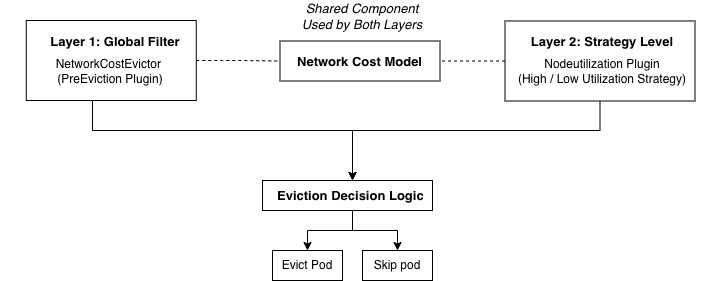
\includegraphics[width=1.0\textwidth]{assets/pics/network-aware/sysoverview-diagram.png}
	\caption{Network-Aware plugin high-level design.}
	\label{fig:netaware_sysoverview}
\end{figure}

The overall design of the Network-Aware Descheduler plugin is presented in Figure \ref{fig:netaware_sysoverview}. The system has two distinct independent components that can be deployed optionally as descheduler policy. 

The first component is a global PreEvictionFilter plugin, which is the \textit{NetworkCostEvictor}. To avoid descheduler process resulting higher network costs, it compares eviction candidates current node with all ready nodes in the cluster. This ensures that the communication efficiency at the cluster level is not degraded due to pod migration. 

The second plugin is integrated into node utilization based approaches, such as \textit{LowNodeUtilization} and \textit{HighNodeUtilization}. This plugin performs network-aware filtering by assessing only the selected subset of nodes that are recognized as potential destinations (e.g. overutilize/underutilize node). This enables a more specific evaluation better aligned with the resource balancing goals of the descheduler. 

Both components use a network cost model \ref{sec:netaware_costmodel} to estimate communication costs between pods. During the eviction process, the algorithm evaluates the cost of the pod's current placement in comparison to alternative placements. If the eviction does not maintain or improve the performance of the network, it is blocked. Otherwise, the eviction is permitted.

%----------------------------------------------------------------------------- %%
\subsection{Architecture Design}
\label{sec:netaware_arcdesign}
%----------------------------------------------------------------------------- %%
\begin{figure}
	\centering
	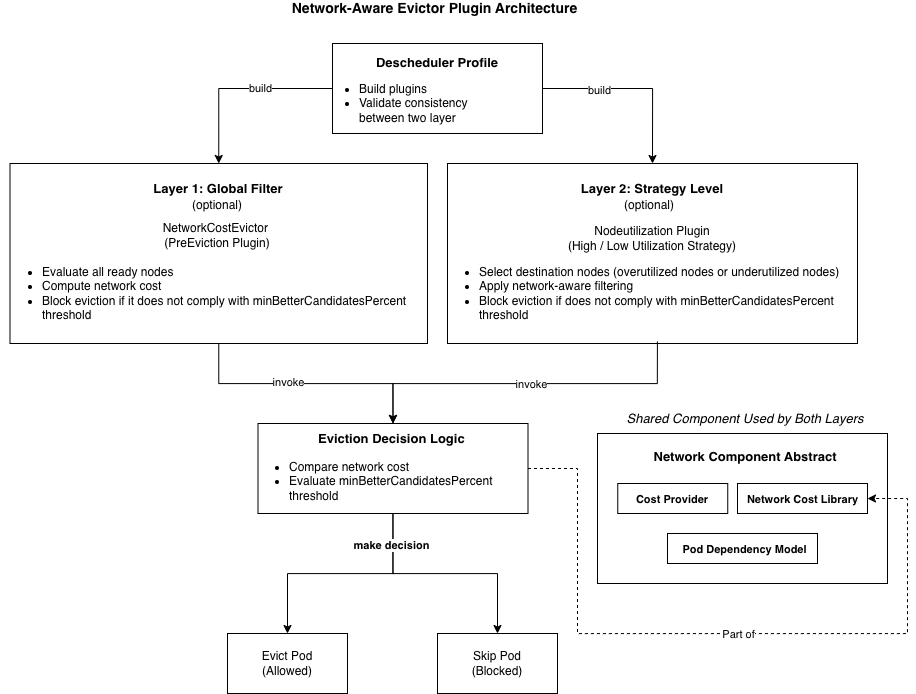
\includegraphics[width=1.0\textwidth]{assets/pics/network-aware/sysarc-diagram.png}
	\caption{Network-Aware plugin architecture design.}
	\label{fig:netaware_arcdesign}
\end{figure}

The detailed architecture of the Network-Aware Descheduler plugin is shown in Figure \ref{fig:netaware_arcdesign} based on the system overview described in Section \ref{sec:netaware_sysoverview}. The architecture enhances the descheduler eviction process with a common network-aware assessment scheme that is uniformly applied to the architectural levels. 

To support this design, the system is structured around three core components. The first component is the Network Cost Model abstracted into Cost Provider, which describes the calculation of the network distance between nodes. The abstraction enables topology-aware estimation based on node locality like region and zone, and latency-aware estimation based on real-time data collected via Prometheus. 

The second component is the Pod Dependency Model, which enables the system to estimate the cost of communication considering interdependent workloads. This is done by a labeling method, where pods with the same configuration label (by default \textit{network-group}) value are grouped together and regarded as a close dependency in the cost calculation. 

The third component is Shared Network Cost Library, the centralized implementation for cost computation and the eviction decision maker. Both architectural layers use this library to ensure that the same logic is used to analyze network cost, regardless of the scope of evaluation. 

The eviction decision itself is based on a common evaluation mechanism. The candidate nodes set is different between layers (from all ready nodes to strategy selected subsets), but the same decision mechanism is utilized. 

To balance between network latency and resource defragmentation goals, an eviction is allowed only if a given ratio of candidate nodes, which is specified by a configurable threshold, have a network cost lower or equal to ($\leq$) the current placement, otherwise the eviction is blocked. This threshold-based solution improves the likelihood of the following scheduling decisions to reschedule pods on nodes that do not degrade the network efficiency and still allow for appropriate workload redistribution. 

\subsection{Network Cost Model}
\label{sec:netaware_costmodel}
%----------------------------------------------------------------------------- %%
To accommodate various deployment situations and accuracy levels, the Network Cost Model employs two distinct methodologies for cost computation: a topology-based cost model and a latency-based cost model. Both methodologies are encompassed inside the Cost Provider abstraction and can be chosen via configuration, as detailed in Chapter \ref{sec:netaware_arcdesign}. The topology-based model offers a lightweight and static assessment, whereas the latency-based model facilitates a dynamic and measurement-driven evaluation grounded in real-time network conditions.
\subsubsection{Topology Base Cost Model}
\label{sec:netaware_topologycostmodel}
%----------------------------------------------------------------------------- %%
The topology-based cost model calculates the network cost based on the node locality information, e.g., zone and region information. This is based on the assumption that the network latency rises with the physical or logical distance of nodes. Thus, the connection between nodes of the same zone is considered cheaper than the communication across zones or regions. 

The model assigns specified costs based on relative position of nodes. A typical arrangement defines three tiers of cost: same-zone, same-region, and cross-region connectivity. For example, the cost of communication between nodes in the same zone is the lowest while the cost of communication across areas is the largest. The model sets defaults cost numbers to reflect this hierarchy: 1 for same-zone, 5 for same-region, 10 for cross-region. These values can be customized through configuration. 

The advantage of this methods is its low processing overhead and independence from external monitoring systems. However, it is based on the simplistic assumption that the network performance is directly proportional to the physical proximity. In practice, this assumption may not always hold, as network latency might be altered by dynamic factors such as node load, congestion, or infrastructure variations.  Nodes within the same zone can sometimes have higher latency than nodes in separate regions. 

However, the topology-based model is a useful baseline for network-aware scheduling when real-time latency information is not accessible or not needed.

\subsubsection{Latency Base Cost Model}
\label{sec:netaware_latencycostmodel}

The latency-based cost model computes the network cost according to the observed node-to-node communication performance, which can provide a more accurate representation of the network conditions by considering the real-time latency between nodes and can adapt to the dynamic changes in the cluster environment by capturing temporary factors like network congestion or unequal workload allocation, which may dramatically affect the communication performance.

To support this capability the system is integrated with a Prometheus based monitoring infrastructure that provides the latency metrics. The user must provide a Prometheus endpoint and a query for fetching node-to-node latency details. Latency numbers are usually derived from aggregated data across a certain time window (e.g. the average response time between nodes).

\begin{figure}
	\centering
	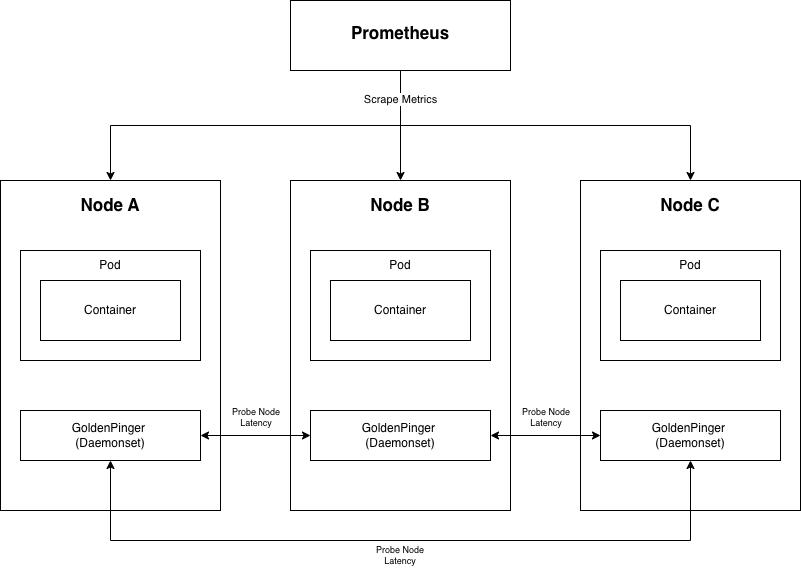
\includegraphics[width=1.0\textwidth]{assets/pics/network-aware/prometheus-scrape.png}
	\caption{Prometheus scraping architecture for inter-node latency metrics via GoldenPinger DaemonSets.}
	\label{fig:netaware_prometheusscrape}
\end{figure}

As seen in Figure \ref{fig:netaware_prometheusscrape}. In this architecture, Goldenpinger is employed as the probing tool to test the node-to-node latency across the cluster. Each node runs an instance of Goldenpinger, which actively probes other nodes and exposes the resulting latency measurements. Prometheus then scrapes these parameters on a regular basis and stores them as time-series data. This version uses Goldenpinger but any other tool that is able to collect latency data and expose it in a Prometheus compatible format can be used.

Besides the query description, the configuration has to define the mapping between metric labels and cluster nodes. In particular, the latency measurements are associated with the respective source and target node labels. This enables the system to create a delay matrix that specifies the communication cost between the nodes.

%----------------------------------------------------------------------------- %%
\subsubsection{Consistency Between Layers}
\label{sec:netaware_costmodelconsistency}
%----------------------------------------------------------------------------- %%
The proposed architecture enforces consistency between the global PreEvictionFilter and the strategy-level component through profile-level configuration validation. Although each plugin exposes its own set of configurable parameters including threshold values, dependency labels, and cost model settings, specific elements related to network cost computation must remain aligned when both components are enabled within the same descheduler profile. 

In particular, the selection of the cost evaluation approach must be consistent across both layers. When latency based cost evaluation is selected, both components are required to utilize identical Prometheus query definitions and consistent node label mappings, such as the source and target node identifiers. This ensures that network cost is derived from the same underlying observations and measurement semantics. Similarly, the dependency identification mechanism, defined through the \textit{network-group} label, must be consistently configured to guarantee uniform grouping of interdependent pods during cost evaluation.

An exception to this requirement is the threshold parameter (e.g., \textit{minBetterCandidatesPercent}), which may be configured independently for each component. This allows different levels of strictness to be applied at the global filtering stage and the strategy-level evaluation.

If any inconsistency is detected in the cost model configuration, the system performs validation at the profile level and raises an error. This design ensures that both components operate within a consistent cost model, thereby preventing discrepancies in cost evaluation that could otherwise lead to conflicting eviction decisions. The corresponding configuration parameters are presented in Section \ref{sec:netaware_config}.



%----------------------------------------------------------------------------- %%
\subsection{Eviction Decision Workflow and Algorithm}
\label{sec:netaware_algorithm}
%----------------------------------------------------------------------------- %%
\begin{figure}
	\centering
	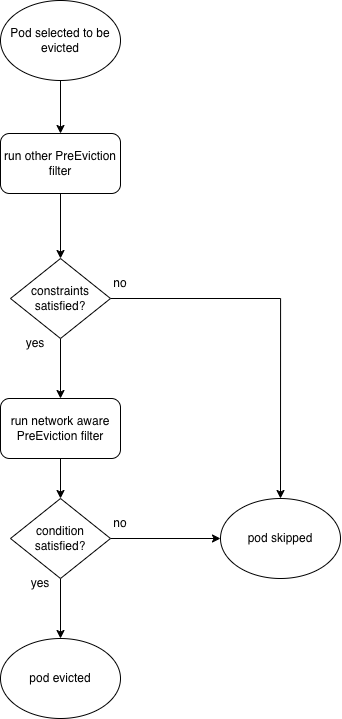
\includegraphics[width=0.3\textwidth]{assets/pics/network-aware/preevict-chaining.png}
	\caption{Pre-eviction filter chaining.}
	\label{fig:netaware_preevictchaining}
\end{figure}

The network-aware eviction decision workflow is implemented within the chaining of descheduler pre-eviction plugins. As shown in Figure \ref{fig:netaware_preevictchaining}, each candidate pod for eviction undergoes a chain of filtering processes before the actual eviction.

The first stage is the built-in \textit{DefaultEvictor} plugin provided by the Kubernetes descheduler framework. This component evaluates several default eviction constraints such as pod state validation, scheduling constraints and node fit requirements to ensure that the pod is eligible for eviction \citep{k8s_descheduler_docs}. If any of these constraints is violated the eviction procedure is cancelled and the pod is skipped. Otherwise the eviction candidate continues to the next phase. 

After passing the default pre-eviction filtering stage,the proposed Network-Aware Evictor plugin conducts an additional network-aware evaluation, as seen in Listing \ref{lst:netaware_unified_algorithm}. This stage determines whether the eviction is expected to preserve or improve the efficiency of network connectivity in the cluster. 

\lstinputlisting[
    caption={Network-aware algorithm}, 
    label={lst:netaware_unified_algorithm},
]{assets/codes/pseudos/netaware-unifiedalgo.psu}

During the network-aware evaluation phase, the system first initializes the network cost provider used for communication cost computation. If latency metrics are configured, the plugin queries Prometheus to obtain node-to-node latency measurements and constructs a latency-based cost provider. Otherwise, the system falls back to the topology-based cost provider, which estimates communication cost using predefined topology distances such as zone and region locality.

When the strategy-level component is enabled, the system additionally classifies cluster nodes according to their utilization state. Resource utilization is computed by comparing the total requested resources on each node against the allocatable node capacity. Nodes whose utilization exceeds the configured target threshold are classified as overutilized nodes, whereas nodes below the lower utilization threshold are classified as underutilized nodes. Depending on the selected balancing strategy, the candidate destination set is then derived from either the overutilized or underutilized node group. In contrast, the global filtering layer evaluates all ready nodes in the cluster as potential destination candidates.

For each selected eviction candidate pod, the algorithm first checks whether the pod contains the configured dependency label. If no dependency label is present, the eviction is immediately permitted because no communication dependency needs to be preserved. Otherwise, the system identifies all dependent pods belonging to the same communication group using the \textit{FindDependencyPods} function shown in Listing \ref{lst:netaware_finddeppods_algo}.

\lstinputlisting[
    caption={\textit{FindDependencyPods} function}, 
    label={lst:netaware_finddeppods_algo}, 
]{assets/codes/pseudos/netaware-finddeppods.psu}
\lstinputlisting[
    caption={\textit{HasSameOwner} function}, 
    label={lst:netaware_hasowner_algo}, 
]{assets/codes/pseudos/netaware-hasowner.psu}

The \textit{FindDependencyPods} function discovers communication dependencies by examining all pods across cluster nodes and comparing their configured dependency labels. Pods sharing the same dependency label are considered part of the same communication group. During this process, the algorithm excludes the evaluated pod itself and may optionally exclude pods managed by the same controller, such as replicas belonging to the same Deployment, StatefulSet, or ReplicaSet by evaluating \textit{HasSameOwner} function shown in Listing \ref{lst:netaware_hasowner_algo}. This behavior is controlled through the \textit{excludeSameOwner} configuration parameter. The ownership relationship is determined by comparing Kubernetes owner references between pods.

After dependency discovery, the algorithm computes the communication cost between the evaluated pod and all dependency pods using the \textit{ComputePlacementCost} procedure shown in Listing \ref{lst:netaware_computeplacement_algo}. This procedure evaluates the communication cost for both the current node placement and all candidate destination nodes. The set of evaluated candidate nodes depends on the architectural layer being used. The global filtering layer evaluates all ready nodes in the cluster, whereas the strategy-level layer evaluates only the nodes selected by the balancing strategy.

\lstinputlisting[
    caption={\textit{ComputePlacementCost} function}, 
    label={lst:netaware_computeplacement_algo}, 
]{assets/codes/pseudos/netaware-computecost.psu}

The network cost calculation performed by the \textit{ComputePlacementCost} procedure is formally defined in Equation (\ref{eq:networkcost}). Given a candidate pod $P$ residing on node $n$, the total communication cost is calculated as the summation of network costs between node $n$ and the nodes hosting all dependency pods $d \in D$.

\begin{equation}
\func{Cost}{n, P} = \sum_{d \in D} \func{Network}{n, \text{Node}_{d}}
\label{eq:networkcost}
\end{equation}

The \textit{ComputePlacementCost} procedure iterates through all dependency pods and retrieves the node hosting each dependency pod. Using the configured cost provider, the algorithm computes the pairwise communication cost between the candidate destination node and each dependency node. The resulting costs are accumulated to produce the total placement cost for the evaluated node.

After computing the communication cost for the current placement and all candidate nodes, the algorithm evaluates whether the eviction satisfies the configured threshold condition. For each candidate node, the computed candidate cost is compared against the current placement cost. The system then counts the number of candidate nodes whose communication cost is lower than or equal to the current placement cost.

The eviction decision is determined using the threshold condition defined in Equation (\ref{eq:networkthreshold}).

\begin{equation}
{\text{Count}(\text{Cost}(C, P) \leq \text{Cost}(a, P))}
\geq
{\text{TotalCandidates}} \cdot \text{MinBetterCandidatesPercent}
\label{eq:networkthreshold}
\end{equation}

An eviction is permitted only if the number of candidate nodes satisfying the condition exceeds the minimum threshold defined by \textit{MinBetterCandidatesPercent}, which defaults to 50\%. Otherwise, the eviction is rejected.

This threshold-based mechanism is intended to balance workload redistribution objectives with communication efficiency. By requiring a sufficient proportion of candidate nodes to maintain or improve network cost, the algorithm increases the likelihood that the Kubernetes scheduler will subsequently place the evicted pod onto a node that preserves or improves network locality after rescheduling.

%----------------------------------------------------------------------------- %%
\subsection{Plugin Configuration}
\label{sec:netaware_config}
%----------------------------------------------------------------------------- %%
The configuration structure of the proposed Network-Aware Descheduler policy consists of two independent configuration corresponding to the two layers architectural components discussed in Section \ref{sec:netaware_sysoverview} and \ref{sec:netaware_arcdesign}. The first layer configures the global \textit{NetworkCostEvictor} plugin operating at the \textit{PreEvictionFilter} phases, while the second layer extends node utilization balancing strategies with network-aware evaluation capabilities.

\lstinputlisting[
    caption={Layer 1: Global preEvictionFilter configuration}, 
    label={lst:netaware_l1config},
]{assets/codes/pseudos/netaware-configL1.psu}

Listing \ref{lst:netaware_l1config} show the \textit{NetworkCostEvictor} configuration that defines the behavior of the global network-aware filtering mechanism. This component evaluates candidate pod evictions against all ready nodes in the cluster before the eviction is permitted. The configuration includes parameters for dependency identification, minimum threshold percentage, pods ownership filtering flag, and optional latency-based cost evaluation through Prometheus metrics.

The \textit{networkGroupLabelKey} parameter specifies the label key used to identify communication groups between pods. Pods sharing the same label value are treated as interdependent workloads during network cost evaluation. The \textit{minBetterCandidatesPercent} parameter controls the strictness of the global filtering stage by defining the minimum percentage of candidate nodes that must provide a lower or equal communication cost before eviction is allowed. The \textit{excludeSameOwner} parameter determines whether replicas managed by the same Kubernetes controller are excluded from dependency discovery.

The optional \textit{latencyMetrics} section enables latency-based communication cost evaluation using Prometheus metrics. The configuration defines the PromQL query used to retrieve node-to-node latency measurements together with the source and destination node label mappings required to construct the latency matrix used during cost evaluation.

\lstinputlisting[
    caption={Layer 2: NodeUtilization extended configuration}, 
    label={lst:netaware_l2config},
]{assets/codes/pseudos/netaware-configL2.psu}

The second configuration \ref{lst:netaware_l2config} extends node utilization strategies such as \textit{LowNodeUtilization} and \textit{HighNodeUtilization} with network-aware filtering capabilities. In addition to the standard resource balancing parameters such as \textit{thresholds} and \textit{targetThresholds}, the strategy exposes an optional \textit{networkAware} configuration block. When this block is removed, the strategy behaves identically to the default Kubernetes descheduler implementation without network-aware evaluation.

The \textit{networkAware} section defines the network cost evaluation behavior used during the strategy-level eviction filtering stage. Similar to the global filtering layer, this configuration supports dependency identification, minimum threshold percentage, pods ownership filtering flag, and multiple cost evaluation approaches. Unlike the global filtering layer, however, the strategy-level component evaluates only the subset of candidate destination nodes selected by the balancing strategy rather than all ready nodes in the cluster.

The configuration supports two mutually exclusive cost evaluation modes: \textit{topologyBase} and \textit{latencyBase}. The topology-based mode uses predefined locality weights without the need for any external monitoring infrastructure, whereas the latency-based mode derives communication cost from real-time Prometheus metrics. When latency-based evaluation is enabled, the configuration must additionally provide the Prometheus query and node label mappings required to retrieve node-to-node latency measurements.

As discussed in Section \ref{sec:netaware_costmodelconsistency}, several configuration parameters must remain consistent when both architectural layers are enabled at the same time within the same descheduler profile. In particular, the dependency label configuration, the selected cost evaluation model, the Prometheus query definition, and the source and destination node label mappings must be identical across both layers. This ensures that both components evaluate network cost using the same communication model and underlying latency data. 

The only exception to this consistency requirement is the \textit{minBetterCandidatesPercent} parameter, which may be configured differently for each layer. This enables the global filtering stage and the strategy-level filtering stage to apply different levels of strictness during eviction evaluation. The system validates these configuration constraints during profile initialization and rejects invalid configurations that could result in inconsistent network cost evaluation behaviour between architectural layers.

